\documentclass{article}
\usepackage{pgf}
\usepackage{pgfpages}

% Options for packages loaded elsewhere
\PassOptionsToPackage{unicode}{hyperref}
\PassOptionsToPackage{hyphens}{url}
%

\usepackage{amsmath,amssymb}
\usepackage{lmodern}
\usepackage{iftex}
\ifPDFTeX
\usepackage[T1]{fontenc}
\usepackage[utf8]{inputenc}
\usepackage{pythontex}
\usepackage{textcomp} % provide euro and other symbols
\else % if luatex or xetex
\usepackage{unicode-math}
\defaultfontfeatures{Scale=MatchLowercase}
\defaultfontfeatures[\rmfamily]{Ligatures=TeX,Scale=1}
\fi
% Use upquote if available, for straight quotes in verbatim environments
\IfFileExists{upquote.sty}{\usepackage{upquote}}{}
\IfFileExists{microtype.sty}{% use microtype if available
	\usepackage[]{microtype}
	\UseMicrotypeSet[protrusion]{basicmath} % disable protrusion for tt fonts
}{}
\makeatletter
\@ifundefined{KOMAClassName}{% if non-KOMA class
	\IfFileExists{parskip.sty}{%
		\usepackage{parskip}
	}{% else
		\setlength{\parindent}{0pt}
		\setlength{\parskip}{6pt plus 2pt minus 1pt}}
}{% if KOMA class
	\KOMAoptions{parskip=half}}
\makeatother
\usepackage{xcolor}
\IfFileExists{xurl.sty}{\usepackage{xurl}}{} % add URL line breaks if available
\IfFileExists{bookmark.sty}{\usepackage{bookmark}}{\usepackage{hyperref}}
\hypersetup{
	hidelinks,
	pdfcreator={LaTeX via pandoc}}
\urlstyle{same} % disable monospaced font for URLs
\usepackage{color}
\usepackage{fancyvrb}
\newcommand{\VerbBar}{|}
\newcommand{\VERB}{\Verb[commandchars=\\\{\}]}
\DefineVerbatimEnvironment{Highlighting}{Verbatim}{commandchars=\\\{\}}
% Add ',fontsize=\small' for more characters per line
\newenvironment{Shaded}{}{}
\newcommand{\AlertTok}[1]{\textcolor[rgb]{1.00,0.00,0.00}{\textbf{#1}}}
\newcommand{\AnnotationTok}[1]{\textcolor[rgb]{0.38,0.63,0.69}{\textbf{\textit{#1}}}}
\newcommand{\AttributeTok}[1]{\textcolor[rgb]{0.49,0.56,0.16}{#1}}
\newcommand{\BaseNTok}[1]{\textcolor[rgb]{0.25,0.63,0.44}{#1}}
\newcommand{\BuiltInTok}[1]{#1}
\newcommand{\CharTok}[1]{\textcolor[rgb]{0.25,0.44,0.63}{#1}}
\newcommand{\CommentTok}[1]{\textcolor[rgb]{0.38,0.63,0.69}{\textit{#1}}}
\newcommand{\CommentVarTok}[1]{\textcolor[rgb]{0.38,0.63,0.69}{\textbf{\textit{#1}}}}
\newcommand{\ConstantTok}[1]{\textcolor[rgb]{0.53,0.00,0.00}{#1}}
\newcommand{\ControlFlowTok}[1]{\textcolor[rgb]{0.00,0.44,0.13}{\textbf{#1}}}
\newcommand{\DataTypeTok}[1]{\textcolor[rgb]{0.56,0.13,0.00}{#1}}
\newcommand{\DecValTok}[1]{\textcolor[rgb]{0.25,0.63,0.44}{#1}}
\newcommand{\DocumentationTok}[1]{\textcolor[rgb]{0.73,0.13,0.13}{\textit{#1}}}
\newcommand{\ErrorTok}[1]{\textcolor[rgb]{1.00,0.00,0.00}{\textbf{#1}}}
\newcommand{\ExtensionTok}[1]{#1}
\newcommand{\FloatTok}[1]{\textcolor[rgb]{0.25,0.63,0.44}{#1}}
\newcommand{\FunctionTok}[1]{\textcolor[rgb]{0.02,0.16,0.49}{#1}}
\newcommand{\ImportTok}[1]{#1}
\newcommand{\InformationTok}[1]{\textcolor[rgb]{0.38,0.63,0.69}{\textbf{\textit{#1}}}}
\newcommand{\KeywordTok}[1]{\textcolor[rgb]{0.00,0.44,0.13}{\textbf{#1}}}
\newcommand{\NormalTok}[1]{#1}
\newcommand{\OperatorTok}[1]{\textcolor[rgb]{0.40,0.40,0.40}{#1}}
\newcommand{\OtherTok}[1]{\textcolor[rgb]{0.00,0.44,0.13}{#1}}
\newcommand{\PreprocessorTok}[1]{\textcolor[rgb]{0.74,0.48,0.00}{#1}}
\newcommand{\RegionMarkerTok}[1]{#1}
\newcommand{\SpecialCharTok}[1]{\textcolor[rgb]{0.25,0.44,0.63}{#1}}
\newcommand{\SpecialStringTok}[1]{\textcolor[rgb]{0.73,0.40,0.53}{#1}}
\newcommand{\StringTok}[1]{\textcolor[rgb]{0.25,0.44,0.63}{#1}}
\newcommand{\VariableTok}[1]{\textcolor[rgb]{0.10,0.09,0.49}{#1}}
\newcommand{\VerbatimStringTok}[1]{\textcolor[rgb]{0.25,0.44,0.63}{#1}}
\newcommand{\WarningTok}[1]{\textcolor[rgb]{0.38,0.63,0.69}{\textbf{\textit{#1}}}}
\setlength{\emergencystretch}{3em} % prevent overfull lines
\providecommand{\tightlist}{%
	\setlength{\itemsep}{0pt}\setlength{\parskip}{0pt}}
\setcounter{secnumdepth}{-\maxdimen} % remove section numbering
\ifLuaTeX
\usepackage{selnolig}  % disable illegal ligatures
\fi


\pgfpagesdeclarelayout{boxed}
{
	\edef\pgfpageoptionborder{0pt}
}
{
	\pgfpagesphysicalpageoptions
	{%
		logical pages=1,%
	}
	\pgfpageslogicalpageoptions{1}
	{
		border code=\pgfsetlinewidth{2pt}\pgfstroke,%
		border shrink=\pgfpageoptionborder,%
		resized width=.95\pgfphysicalwidth,%
		resized height=.95\pgfphysicalheight,%
		center=\pgfpoint{.5\pgfphysicalwidth}{.5\pgfphysicalheight}%
	}%
}



\pgfpagesuselayout{boxed}
\usepackage{url}
\usepackage{authblk}
\usepackage{amsmath}
\usepackage{setspace}\doublespacing
\usepackage{graphicx} 
\usepackage{amssymb}


\usepackage{amsfonts}
\usepackage{amssymb}
\usepackage{floatflt}
\usepackage{lipsum}
%\usepackage[demo]{graphicx}
\usepackage{upquote} % Upright quotes for verbatim code
\usepackage{eurosym} % defines \euro
\usepackage[mathletters]{ucs} % Extended unicode (utf-8) support
\usepackage[utf8x]{inputenc} % Allow utf-8 characters in the tex document
\usepackage{fancyvrb} % verbatim replacement that allows latex
\usepackage{grffile} % extends the file name processing of package graphics 
\usepackage{xepersian}

\DefineVerbatimEnvironment{Highlighting}{Verbatim}{commandchars=\\\{\}}
% Pygments definitions

\makeatletter
\def\PY@reset{\let\PY@it=\relax \let\PY@bf=\relax%
	\let\PY@ul=\relax \let\PY@tc=\relax%
	\let\PY@bc=\relax \let\PY@ff=\relax}
\def\PY@tok#1{\csname PY@tok@#1\endcsname}
\def\PY@toks#1+{\ifx\relax#1\empty\else%
	\PY@tok{#1}\expandafter\PY@toks\fi}
\def\PY@do#1{\PY@bc{\PY@tc{\PY@ul{%
				\PY@it{\PY@bf{\PY@ff{#1}}}}}}}
\def\PY#1#2{\PY@reset\PY@toks#1+\relax+\PY@do{#2}}

\expandafter\def\csname PY@tok@w\endcsname{\def\PY@tc##1{\textcolor[rgb]{0.73,0.73,0.73}{##1}}}
\expandafter\def\csname PY@tok@c\endcsname{\let\PY@it=\textit\def\PY@tc##1{\textcolor[rgb]{0.25,0.50,0.50}{##1}}}
\expandafter\def\csname PY@tok@cp\endcsname{\def\PY@tc##1{\textcolor[rgb]{0.74,0.48,0.00}{##1}}}
\expandafter\def\csname PY@tok@k\endcsname{\let\PY@bf=\textbf\def\PY@tc##1{\textcolor[rgb]{0.00,0.50,0.00}{##1}}}
\expandafter\def\csname PY@tok@kp\endcsname{\def\PY@tc##1{\textcolor[rgb]{0.00,0.50,0.00}{##1}}}
\expandafter\def\csname PY@tok@kt\endcsname{\def\PY@tc##1{\textcolor[rgb]{0.69,0.00,0.25}{##1}}}
\expandafter\def\csname PY@tok@o\endcsname{\def\PY@tc##1{\textcolor[rgb]{0.40,0.40,0.40}{##1}}}
\expandafter\def\csname PY@tok@ow\endcsname{\let\PY@bf=\textbf\def\PY@tc##1{\textcolor[rgb]{0.67,0.13,1.00}{##1}}}
\expandafter\def\csname PY@tok@nb\endcsname{\def\PY@tc##1{\textcolor[rgb]{0.00,0.50,0.00}{##1}}}
\expandafter\def\csname PY@tok@nf\endcsname{\def\PY@tc##1{\textcolor[rgb]{0.00,0.00,1.00}{##1}}}
\expandafter\def\csname PY@tok@nc\endcsname{\let\PY@bf=\textbf\def\PY@tc##1{\textcolor[rgb]{0.00,0.00,1.00}{##1}}}
\expandafter\def\csname PY@tok@nn\endcsname{\let\PY@bf=\textbf\def\PY@tc##1{\textcolor[rgb]{0.00,0.00,1.00}{##1}}}
\expandafter\def\csname PY@tok@ne\endcsname{\let\PY@bf=\textbf\def\PY@tc##1{\textcolor[rgb]{0.82,0.25,0.23}{##1}}}
\expandafter\def\csname PY@tok@nv\endcsname{\def\PY@tc##1{\textcolor[rgb]{0.10,0.09,0.49}{##1}}}
\expandafter\def\csname PY@tok@no\endcsname{\def\PY@tc##1{\textcolor[rgb]{0.53,0.00,0.00}{##1}}}
\expandafter\def\csname PY@tok@nl\endcsname{\def\PY@tc##1{\textcolor[rgb]{0.63,0.63,0.00}{##1}}}
\expandafter\def\csname PY@tok@ni\endcsname{\let\PY@bf=\textbf\def\PY@tc##1{\textcolor[rgb]{0.60,0.60,0.60}{##1}}}
\expandafter\def\csname PY@tok@na\endcsname{\def\PY@tc##1{\textcolor[rgb]{0.49,0.56,0.16}{##1}}}
\expandafter\def\csname PY@tok@nt\endcsname{\let\PY@bf=\textbf\def\PY@tc##1{\textcolor[rgb]{0.00,0.50,0.00}{##1}}}
\expandafter\def\csname PY@tok@nd\endcsname{\def\PY@tc##1{\textcolor[rgb]{0.67,0.13,1.00}{##1}}}
\expandafter\def\csname PY@tok@s\endcsname{\def\PY@tc##1{\textcolor[rgb]{0.73,0.13,0.13}{##1}}}
\expandafter\def\csname PY@tok@sd\endcsname{\let\PY@it=\textit\def\PY@tc##1{\textcolor[rgb]{0.73,0.13,0.13}{##1}}}
\expandafter\def\csname PY@tok@si\endcsname{\let\PY@bf=\textbf\def\PY@tc##1{\textcolor[rgb]{0.73,0.40,0.53}{##1}}}
\expandafter\def\csname PY@tok@se\endcsname{\let\PY@bf=\textbf\def\PY@tc##1{\textcolor[rgb]{0.73,0.40,0.13}{##1}}}
\expandafter\def\csname PY@tok@sr\endcsname{\def\PY@tc##1{\textcolor[rgb]{0.73,0.40,0.53}{##1}}}
\expandafter\def\csname PY@tok@ss\endcsname{\def\PY@tc##1{\textcolor[rgb]{0.10,0.09,0.49}{##1}}}
\expandafter\def\csname PY@tok@sx\endcsname{\def\PY@tc##1{\textcolor[rgb]{0.00,0.50,0.00}{##1}}}
\expandafter\def\csname PY@tok@m\endcsname{\def\PY@tc##1{\textcolor[rgb]{0.40,0.40,0.40}{##1}}}
\expandafter\def\csname PY@tok@gh\endcsname{\let\PY@bf=\textbf\def\PY@tc##1{\textcolor[rgb]{0.00,0.00,0.50}{##1}}}
\expandafter\def\csname PY@tok@gu\endcsname{\let\PY@bf=\textbf\def\PY@tc##1{\textcolor[rgb]{0.50,0.00,0.50}{##1}}}
\expandafter\def\csname PY@tok@gd\endcsname{\def\PY@tc##1{\textcolor[rgb]{0.63,0.00,0.00}{##1}}}
\expandafter\def\csname PY@tok@gi\endcsname{\def\PY@tc##1{\textcolor[rgb]{0.00,0.63,0.00}{##1}}}
\expandafter\def\csname PY@tok@gr\endcsname{\def\PY@tc##1{\textcolor[rgb]{1.00,0.00,0.00}{##1}}}
\expandafter\def\csname PY@tok@ge\endcsname{\let\PY@it=\textit}
\expandafter\def\csname PY@tok@gs\endcsname{\let\PY@bf=\textbf}
\expandafter\def\csname PY@tok@gp\endcsname{\let\PY@bf=\textbf\def\PY@tc##1{\textcolor[rgb]{0.00,0.00,0.50}{##1}}}
\expandafter\def\csname PY@tok@go\endcsname{\def\PY@tc##1{\textcolor[rgb]{0.53,0.53,0.53}{##1}}}
\expandafter\def\csname PY@tok@gt\endcsname{\def\PY@tc##1{\textcolor[rgb]{0.00,0.27,0.87}{##1}}}
\expandafter\def\csname PY@tok@err\endcsname{\def\PY@bc##1{\setlength{\fboxsep}{0pt}\fcolorbox[rgb]{1.00,0.00,0.00}{1,1,1}{\strut ##1}}}
\expandafter\def\csname PY@tok@kc\endcsname{\let\PY@bf=\textbf\def\PY@tc##1{\textcolor[rgb]{0.00,0.50,0.00}{##1}}}
\expandafter\def\csname PY@tok@kd\endcsname{\let\PY@bf=\textbf\def\PY@tc##1{\textcolor[rgb]{0.00,0.50,0.00}{##1}}}
\expandafter\def\csname PY@tok@kn\endcsname{\let\PY@bf=\textbf\def\PY@tc##1{\textcolor[rgb]{0.00,0.50,0.00}{##1}}}
\expandafter\def\csname PY@tok@kr\endcsname{\let\PY@bf=\textbf\def\PY@tc##1{\textcolor[rgb]{0.00,0.50,0.00}{##1}}}
\expandafter\def\csname PY@tok@bp\endcsname{\def\PY@tc##1{\textcolor[rgb]{0.00,0.50,0.00}{##1}}}
\expandafter\def\csname PY@tok@fm\endcsname{\def\PY@tc##1{\textcolor[rgb]{0.00,0.00,1.00}{##1}}}
\expandafter\def\csname PY@tok@vc\endcsname{\def\PY@tc##1{\textcolor[rgb]{0.10,0.09,0.49}{##1}}}
\expandafter\def\csname PY@tok@vg\endcsname{\def\PY@tc##1{\textcolor[rgb]{0.10,0.09,0.49}{##1}}}
\expandafter\def\csname PY@tok@vi\endcsname{\def\PY@tc##1{\textcolor[rgb]{0.10,0.09,0.49}{##1}}}
\expandafter\def\csname PY@tok@vm\endcsname{\def\PY@tc##1{\textcolor[rgb]{0.10,0.09,0.49}{##1}}}
\expandafter\def\csname PY@tok@sa\endcsname{\def\PY@tc##1{\textcolor[rgb]{0.73,0.13,0.13}{##1}}}
\expandafter\def\csname PY@tok@sb\endcsname{\def\PY@tc##1{\textcolor[rgb]{0.73,0.13,0.13}{##1}}}
\expandafter\def\csname PY@tok@sc\endcsname{\def\PY@tc##1{\textcolor[rgb]{0.73,0.13,0.13}{##1}}}
\expandafter\def\csname PY@tok@dl\endcsname{\def\PY@tc##1{\textcolor[rgb]{0.73,0.13,0.13}{##1}}}
\expandafter\def\csname PY@tok@s2\endcsname{\def\PY@tc##1{\textcolor[rgb]{0.73,0.13,0.13}{##1}}}
\expandafter\def\csname PY@tok@sh\endcsname{\def\PY@tc##1{\textcolor[rgb]{0.73,0.13,0.13}{##1}}}
\expandafter\def\csname PY@tok@s1\endcsname{\def\PY@tc##1{\textcolor[rgb]{0.73,0.13,0.13}{##1}}}
\expandafter\def\csname PY@tok@mb\endcsname{\def\PY@tc##1{\textcolor[rgb]{0.40,0.40,0.40}{##1}}}
\expandafter\def\csname PY@tok@mf\endcsname{\def\PY@tc##1{\textcolor[rgb]{0.40,0.40,0.40}{##1}}}
\expandafter\def\csname PY@tok@mh\endcsname{\def\PY@tc##1{\textcolor[rgb]{0.40,0.40,0.40}{##1}}}
\expandafter\def\csname PY@tok@mi\endcsname{\def\PY@tc##1{\textcolor[rgb]{0.40,0.40,0.40}{##1}}}
\expandafter\def\csname PY@tok@il\endcsname{\def\PY@tc##1{\textcolor[rgb]{0.40,0.40,0.40}{##1}}}
\expandafter\def\csname PY@tok@mo\endcsname{\def\PY@tc##1{\textcolor[rgb]{0.40,0.40,0.40}{##1}}}
\expandafter\def\csname PY@tok@ch\endcsname{\let\PY@it=\textit\def\PY@tc##1{\textcolor[rgb]{0.25,0.50,0.50}{##1}}}
\expandafter\def\csname PY@tok@cm\endcsname{\let\PY@it=\textit\def\PY@tc##1{\textcolor[rgb]{0.25,0.50,0.50}{##1}}}
\expandafter\def\csname PY@tok@cpf\endcsname{\let\PY@it=\textit\def\PY@tc##1{\textcolor[rgb]{0.25,0.50,0.50}{##1}}}
\expandafter\def\csname PY@tok@c1\endcsname{\let\PY@it=\textit\def\PY@tc##1{\textcolor[rgb]{0.25,0.50,0.50}{##1}}}
\expandafter\def\csname PY@tok@cs\endcsname{\let\PY@it=\textit\def\PY@tc##1{\textcolor[rgb]{0.25,0.50,0.50}{##1}}}

\def\PYZbs{\char`\\}
\def\PYZus{\char`\_}
\def\PYZob{\char`\{}
\def\PYZcb{\char`\}}
\def\PYZca{\char`\^}
\def\PYZam{\char`\&}
\def\PYZlt{\char`\<}
\def\PYZgt{\char`\>}
\def\PYZsh{\char`\#}
\def\PYZpc{\char`\%}
\def\PYZdl{\char`\$}
\def\PYZhy{\char`\-}
\def\PYZsq{\char`\'}
\def\PYZdq{\char`\"}
\def\PYZti{\char`\~}
% for compatibility with earlier versions
\def\PYZat{@}
\def\PYZlb{[}
\def\PYZrb{]}
\makeatother

% Exact colors from NB
\definecolor{incolor}{rgb}{0.0, 0.0, 0.5}
\definecolor{outcolor}{rgb}{0.545, 0.0, 0.0}
\renewcommand\Authsep{، }
\renewcommand\Authands{ و }
\renewcommand\Authand{ و }

\newcommand{\namen}{نام و نام خانوادگی :}
\newcommand{\term}{Spring 2012}
\newcommand{\id}{شماره دانشجویی :}
\newcommand{\examdate}{3/28/12}
\newcommand{\timelimit}{50 Minutes}


\pagestyle{empty}
\addtolength{\textwidth}{7.5cm}
\addtolength{\textheight}{8cm}
\addtolength{\topmargin}{-3.5cm}
\addtolength{\oddsidemargin}{-4cm}
%\addtolength{\evensidemargin}{2cm}
\settextfont[Scale=1]{XB Zar}
\setlatintextfont{Liberation Mono}
%\def\LOGO{%
	%\begin{picture}(0,0)\unitlength=1cm
	%\put (0,-1) {\includegraphics[width=4.9em]{index.png}}
	%\end{picture}
	%}

\begin{document}
	
	\title {ویژگی‌های نیم رساناها: باتری‌ خورشیدی\\
		\vspace{0.5cm}
		\large گروه یک: آقایان سعید شیرانی، آبتین الماسی، امیرسهیل بلوچستان‌زاده\\}
	
	\author{نگارنده: سعید شیرانی} 
%	\author{استاد درس: جناب دکتر مظفری} 
	
	\affil{ }
	\maketitle
	\newpage{}
	\normalsize 
	
	\section{هدف آزمایش}
	\vspace{5mm}
	\normalsize
	
	بررسی تغییرات جریان اتصال کوتاه ($I_{sc}$) با شدت نور‌فرودی، محاسبه‌ی ولتاژ مدار باز($V_{oc}$)، محاسبه‌ی سازه‌ی پرشدگی($FF$)بررسی تغییرات جریان اتصال کوتاه($I_{sc}$) با زاویه‌‌ی فرود(زاویه‌ی میان‌خط عمود برسطح باتری خورشیدی و پرتوی‌فرودی)
	
	\section{ابزار آزمایش:}
	باتری خورشید، ولت‌سنج، آمپرسنج، جعبه مقاومت، چراغ شش ولتی، میزچه مدرج
	\section{چگونگی انجام آزمایش:}
	
	نور چشمه را به گونه‌ای یکنواخت روی باتری خورشیدی بیندازید. \\
	1. جریان  اتصال کوتاه $I_{sc}$ را با بستن آمپرسنج به دوسر باتری خورشیدی(بی‌مقاومت) برحسب فاصله‌ی چشمه از آن اندازه‌بگیرید و در جدول زیر یادداشت کنید. منحنی جریان اتصال کوتاه $I_{sc}$، برحسب فاصله‌ی چشمه از باتری خورشیدی رسم کنید. برای خطی شدن نمودار می‌توان از شدت برحسب یک توان مناسب از فاصله رسم کنید تا رابطه خطی بدست آید. \\
	\textbf{نکته:} با تغییر فاصله‌ی چشمه از باتری خورشیدی، شدت نور تابیده به باتری تغییر می‌کند.
\vspace{3cm}
\begin{center}
\begin{table}[h!]
\centering

\setlength{\tabcolsep}{20pt}
\renewcommand{\arraystretch}{2}

\begin{tabular}{|c|c|}
\hline
\centering
$I_{sc} (mA)$ & \rl{ فاصله(cm)  \pm $0.1$ cm}\\
\hline
\hline
$0.105\pm0.004$ & $90$ \\ 
\hline
$0.118\pm0.002$ & $85$ \\
\hline
$0.128\pm0.002$ & $80$ \\
\hline
$0.142\pm0.001$ & $75$ \\
\hline
$0.160\pm0.001$ & $70$ \\
\hline
$0.180\pm0.001$ & $65$ \\
\hline
$0.203\pm0.001$ & $60$ \\
\hline
$0.236\pm0.001$ & $55$ \\
\hline
$0.275\pm0.001$ & $50$ \\
\hline
$0.325\pm0.001$ & $45$ \\
\hline
\end{tabular}
\caption{تغییرات جریان اتصال کوتاه برحسب فاصله‌ی چشمه از باتری خورشیدی}
\end{table}
\end{center}

	\newpage
	
\begin{latin}
\hypertarget{i_sc---distance}{%
\section{\texorpdfstring{\(I_{SC}\) -
Distance}{I\_\{SC\} - Distance}}\label{i_sc---distance}}
\begin{Shaded}
\begin{Highlighting}[]
\CommentTok{\# draw chart I\_sc {-} d }
\CommentTok{\# d with respect to cm}
\CommentTok{\# for get a linear chart we should insert distance in a upper power d\^{}n}
\end{Highlighting}
\end{Shaded}
\begin{Shaded}
\begin{Highlighting}[]
\ImportTok{import}\NormalTok{ matplotlib.pyplot }\ImportTok{as}\NormalTok{ plt}
\ImportTok{import}\NormalTok{ seaborn }\ImportTok{as}\NormalTok{ sns}
\ImportTok{import}\NormalTok{ pandas }\ImportTok{as}\NormalTok{ pd}
\ImportTok{import}\NormalTok{ numpy }\ImportTok{as}\NormalTok{ np}
\ImportTok{import}\NormalTok{ scipy}
\CommentTok{\# create set of data}
\NormalTok{I\_SO }\OperatorTok{=}\NormalTok{ np.array([}\FloatTok{0.105}\NormalTok{, }\FloatTok{0.118}\NormalTok{, }\FloatTok{0.128}\NormalTok{, }\FloatTok{0.142}\NormalTok{, }\FloatTok{0.160}\NormalTok{, }\FloatTok{0.180}\NormalTok{, }\FloatTok{0.203}\NormalTok{, }\FloatTok{0.236}\NormalTok{, }\FloatTok{0.275}\NormalTok{, }\FloatTok{0.325}\NormalTok{]) }\CommentTok{\# IN MILLI AMPER UNIT}
\NormalTok{DISTANCE }\OperatorTok{=}\NormalTok{ np.array([}\FloatTok{0.9}\NormalTok{, }\FloatTok{0.85}\NormalTok{, }\FloatTok{0.80}\NormalTok{, }\FloatTok{0.75}\NormalTok{,}\FloatTok{0.70}\NormalTok{, }\FloatTok{0.65}\NormalTok{, }\FloatTok{0.60}\NormalTok{, }\FloatTok{0.55}\NormalTok{, }\FloatTok{0.50}\NormalTok{, }\FloatTok{0.45}\NormalTok{])}\OperatorTok{**}\FloatTok{0.5} \CommentTok{\# IN METER UNIT}
\NormalTok{df }\OperatorTok{=}\NormalTok{ pd.DataFrame(\{}\StringTok{\textquotesingle{}DISTANCE(m)\textquotesingle{}}\NormalTok{:DISTANCE, }\StringTok{\textquotesingle{}I\_SO(mA)\textquotesingle{}}\NormalTok{:I\_SO\})}
\CommentTok{\#create regplot}
\NormalTok{p }\OperatorTok{=}\NormalTok{ sns.regplot(data}\OperatorTok{=}\NormalTok{df, x}\OperatorTok{=}\NormalTok{df[}\StringTok{\textquotesingle{}DISTANCE(m)\textquotesingle{}}\NormalTok{], y}\OperatorTok{=}\NormalTok{df[}\StringTok{\textquotesingle{}I\_SO(mA)\textquotesingle{}}\NormalTok{])}
\CommentTok{\#calculate slope and intercept of regression equation we use slop and intercept in equation}
\NormalTok{slope, intercept, r, p, sterr }\OperatorTok{=}\NormalTok{ scipy.stats.linregress(x}\OperatorTok{=}\NormalTok{p.get\_lines()[}\DecValTok{0}\NormalTok{].get\_xdata(),}
\NormalTok{                                                       y}\OperatorTok{=}\NormalTok{p.get\_lines()[}\DecValTok{0}\NormalTok{].get\_ydata())}
\CommentTok{\#add regression equation to plot}
\NormalTok{equation1 }\OperatorTok{=} \StringTok{\textquotesingle{}y = \textquotesingle{}} \OperatorTok{+} \BuiltInTok{str}\NormalTok{(}\BuiltInTok{round}\NormalTok{(intercept,}\DecValTok{3}\NormalTok{)) }\OperatorTok{+} \StringTok{\textquotesingle{} + \textquotesingle{}} \OperatorTok{+} \BuiltInTok{str}\NormalTok{(}\BuiltInTok{round}\NormalTok{(slope,}\DecValTok{3}\NormalTok{)) }\OperatorTok{+} \StringTok{\textquotesingle{}x\textquotesingle{}}

\NormalTok{plt.legend()}
\NormalTok{plt.show()}
\end{Highlighting}
\end{Shaded}
\begin{center}
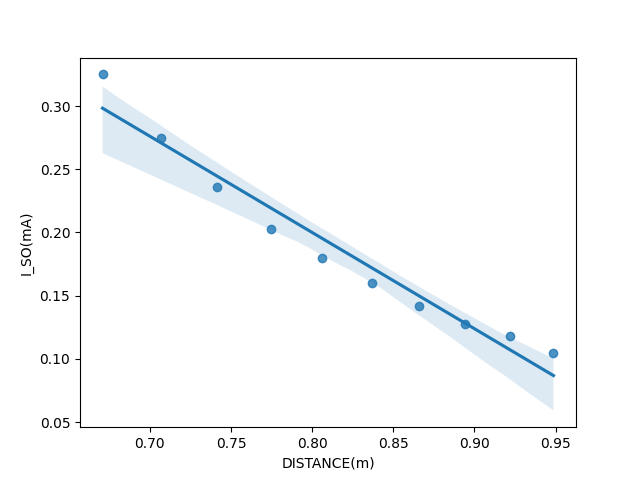
\includegraphics[scale=0.75]{I_SO.png}	
\end{center}
\end{latin}
\newpage

برای آنکه نمودار به صورت خطی شود؛ شدت را برحسب جذر فاصله(توان $\frac{1}{2}$) رسم کردیم.
\begin{latin}
\begin{Highlighting}
\BuiltInTok{print}\NormalTok{(}\SpecialStringTok{F"Eq1: }\SpecialCharTok{\{}\NormalTok{equation1}\SpecialCharTok{\}}\SpecialStringTok{"}\NormalTok{)}
\end{Highlighting}
\end{latin}
معادله‌ی خط فیت شده به شکل زیر است:
\begin{latin}
\begin{verbatim}
Eq1: y = 0.809 + -0.761x
\end{verbatim}
\end{latin}

	2. مدار آزمایش را مانند شکل 3 در دستورکار ببندید.
	
	باتری خورشیدی را در فاصله‌ی ثابت 40 سانتی‌متری قرار می‌دهیم. مقدار جعبه‌ی مقاومت را به صورت لگاریتمی(1, 2, 5, 10, 20, 50, 100, 200, 500, 1000, 2000, 5000) تغییر می‌دهیم تا حاصل ضرب IV بیشینه شود و مقادیر متناظر را در جدول 2 یادداشت می‌کنیم. مقاومت را تاجایی بالا می‌بریم ک دیگر مقدار V تغییری نکند. این $V_{oc}$ است. اینک پیرامون مقاومتی ‌که IV بیشینه است، برای چند مقاومت دیگر (کوچکتر و بزرگتر) I و V را اندازه می‌گیریم. بیشینه‌ی $I*V$ را مشخص می‌کنیم. این مقادیر همان $V_{mpp}$ و $I_{mpp}$ است. نمودار$I-V$برحسب $R$ را رسم کنید و یک منحنی مناسب در آن برازش کنید.
	
	

\begin{latin}
\vspace{1cm}
\begin{center}
\begin{table}[h!]
\centering

\setlength{\tabcolsep}{20pt}
\renewcommand{\arraystretch}{2}

\begin{tabular}{|c|c|c|c|}
\hline
\multicolumn{4}{|c|}{Changes in current and voltage according to the change in resistance in the resistance box} \\
\hline
R($\Omega$) & I(mA) & V & $I*v$\\
\hline
1&$0.40\pm0.01$ &$0.60mV\pm0.1mV$& $2.4000e-04$ \\ 
\hline
2&$0.40\pm0.01$ &$1.00mV\pm0.1mV$& $ 4.0000e-04$ \\
\hline
5&$0.40\pm0.01$ &$2.40mV\pm0.1mV$& $9.6000e-04$ \\
\hline
10&$0.40\pm0.01$ &$4.10mV\pm0.1mV$& $1.6400e-03$ \\
\hline
20&$0.40\pm0.01$ &$8.20mV\pm0.1mV$& $3.2800e-03$ \\
\hline
50&$0.39\pm0.01$ &$20.60mV\pm0.2mV$& $8.0340e-03$ \\
\hline
100&$0.39\pm0.01$ &$7.20mV\pm0.1mV$& $2.8080e-03$ \\
\hline
200&$0.39\pm0.01$ &$46.8mV\pm0.5mV$& $1.8252e-02$ \\
\hline
500&$0.38\pm0.01$ &$166.0mV\pm0.5mV$& $6.3080e-02$ \\
\hline
1000&$0.39\pm0.01$ &$0.39V\pm0.01V$& $1.5210e-01$ \\
\hline
2000&$0.39\pm0.01$ &$0.78V\pm0.01V$& $3.0420e-01$ \\
\hline
5000&$0.36\pm0.01$ &$1.81V\pm0.01V$& $6.5160e-01$ \\
\hline
10000&$0.28\pm0.01$ &$2.82V\pm0.01V$& $7.8960e-01$ \\
\hline
20000&$0.16\pm0.01$ &$3.43V\pm0.01V$& $5.4880e-01$ \\
\hline
50000&$0.07\pm0.01$ &$3.71V\pm0.01V$& $2.5970e-01$ \\
\hline
100000&$0.03\pm0.01$ &$3.80V\pm0.01V$& $1.1400e-01$ \\
\hline
200000&$0.02\pm0.01$ &$3.85V\pm0.01V$& $7.7000e-02$ \\
\hline
500000&$0.01\pm0.01$ &$3.87V\pm0.01V$& $3.8700e-02$ \\
\hline
\end{tabular}
\caption{}
\end{table}
\end{center}
\end{latin}
	\newpage
	منحنی $I-V$ را رسم ‌می‌کنیم و برای نمایش بهتر داده‌ها از داده‌ها لگاریتم می‌‌گیریم: 
\begin{latin}
\hypertarget{iv-r}{%
\section{IV-R}\label{iv-r}}
\hypertarget{now-we-are-going-to-define-our-datasets}{%
\subsubsection{now we are going to define our
datasets}\label{now-we-are-going-to-define-our-datasets}}
\begin{Shaded}
\begin{Highlighting}[]
\CommentTok{\# IN MILLI AMPER UNIT}
\NormalTok{I }\OperatorTok{=}\NormalTok{ np.array([}\FloatTok{0.4}\NormalTok{, }\FloatTok{0.4}\NormalTok{, }\FloatTok{0.4}\NormalTok{, }\FloatTok{0.4}\NormalTok{, }\FloatTok{0.4}\NormalTok{, }\FloatTok{0.39}\NormalTok{, }\FloatTok{0.39}\NormalTok{, }\FloatTok{0.39}\NormalTok{, }\FloatTok{0.38}\NormalTok{, }\FloatTok{0.39}\NormalTok{, }\FloatTok{0.39}\NormalTok{, }\FloatTok{0.36}\NormalTok{, }\FloatTok{0.28}\NormalTok{, }\FloatTok{0.16}\NormalTok{, }\FloatTok{0.07}\NormalTok{, }\FloatTok{0.03}\NormalTok{, }\FloatTok{0.02}\NormalTok{, }\FloatTok{0.01}\NormalTok{])}
\CommentTok{\# IN Volt UNIT}
\NormalTok{V }\OperatorTok{=}\NormalTok{ np.array([}\FloatTok{0.6}\OperatorTok{*}\FloatTok{0.001}\NormalTok{, }\FloatTok{1.0}\OperatorTok{*}\FloatTok{0.001}\NormalTok{, }\FloatTok{2.4}\OperatorTok{*}\FloatTok{0.001}\NormalTok{, }\FloatTok{4.10}\OperatorTok{*}\FloatTok{0.001}\NormalTok{, }\FloatTok{8.20}\OperatorTok{*}\FloatTok{0.001}\NormalTok{, }\FloatTok{20.60}\OperatorTok{*}\FloatTok{0.001}\NormalTok{, }\FloatTok{7.20}\OperatorTok{*}\FloatTok{0.001}\NormalTok{,}
\FloatTok{46.8}\OperatorTok{*}\FloatTok{0.001}\NormalTok{, }\FloatTok{166.0}\OperatorTok{*}\FloatTok{0.001}\NormalTok{, }\FloatTok{0.39}\NormalTok{, }\FloatTok{0.78}\NormalTok{, }\FloatTok{1.81}\NormalTok{, }\FloatTok{2.82}\NormalTok{, }\FloatTok{3.43}\NormalTok{, }\FloatTok{3.71}\NormalTok{, }\FloatTok{3.80}\NormalTok{, }\FloatTok{3.85}\NormalTok{, }\FloatTok{3.87}\NormalTok{])}
\NormalTok{R }\OperatorTok{=}\NormalTok{ np.array([}\DecValTok{1}\NormalTok{, }\DecValTok{2}\NormalTok{, }\DecValTok{5}\NormalTok{, }\DecValTok{10}\NormalTok{, }\DecValTok{20}\NormalTok{, }\DecValTok{50}\NormalTok{, }\DecValTok{100}\NormalTok{, }\DecValTok{200}\NormalTok{, }\DecValTok{500}\NormalTok{, }\DecValTok{1000}\NormalTok{, }\DecValTok{2000}\NormalTok{, }\DecValTok{5000}\NormalTok{, }\DecValTok{10000}\NormalTok{, }\DecValTok{20000}\NormalTok{, }\DecValTok{50000}\NormalTok{, }\DecValTok{100000}\NormalTok{, }\DecValTok{200000}\NormalTok{, }\DecValTok{500000}\NormalTok{])}
\NormalTok{IV }\OperatorTok{=}\NormalTok{ I}\OperatorTok{*}\NormalTok{V}
\end{Highlighting}
\end{Shaded}
\begin{Shaded}
\begin{Highlighting}[]
\ImportTok{import}\NormalTok{ numpy }\ImportTok{as}\NormalTok{ np}
\ImportTok{import}\NormalTok{ matplotlib.pyplot }\ImportTok{as}\NormalTok{ plt}
\ImportTok{from}\NormalTok{ scipy.optimize }\ImportTok{import}\NormalTok{ curve\_fit}
\CommentTok{\#\# x{-}axis for the plot}
\NormalTok{xdata }\OperatorTok{=}\NormalTok{ np.log(R)}
\NormalTok{ydata }\OperatorTok{=}\NormalTok{ np.log(I}\OperatorTok{*}\NormalTok{V)}
\CommentTok{\# Recast xdata and ydata into numpy arrays so we can use their handy features}
\CommentTok{\# Define the Gaussian function}
\KeywordTok{def}\NormalTok{ Gauss(x, A, B):}
\NormalTok{    y }\OperatorTok{=}\NormalTok{ A}\OperatorTok{*}\NormalTok{np.exp(}\OperatorTok{{-}}\DecValTok{1}\OperatorTok{*}\NormalTok{B}\OperatorTok{*}\NormalTok{x}\OperatorTok{**}\DecValTok{2}\NormalTok{)}
\ControlFlowTok{return}\NormalTok{ y}
\NormalTok{parameters, covariance }\OperatorTok{=}\NormalTok{ curve\_fit(Gauss, xdata, ydata)}
\NormalTok{fit\_A }\OperatorTok{=}\NormalTok{ parameters[}\DecValTok{0}\NormalTok{]}
\NormalTok{fit\_B }\OperatorTok{=}\NormalTok{ parameters[}\DecValTok{1}\NormalTok{]}
\NormalTok{fit\_y }\OperatorTok{=}\NormalTok{ Gauss(xdata, fit\_A, fit\_B)}
\NormalTok{plt.plot(xdata, ydata, }\StringTok{\textquotesingle{}o\textquotesingle{}}\NormalTok{, label}\OperatorTok{=}\StringTok{\textquotesingle{}data\textquotesingle{}}\NormalTok{)}
\NormalTok{plt.plot(xdata, fit\_y, }\StringTok{\textquotesingle{}{-}\textquotesingle{}}\NormalTok{, label}\OperatorTok{=}\StringTok{\textquotesingle{}fit\textquotesingle{}}\NormalTok{)}
\NormalTok{plt.legend()}
\end{Highlighting}
\end{Shaded}
\begin{center}
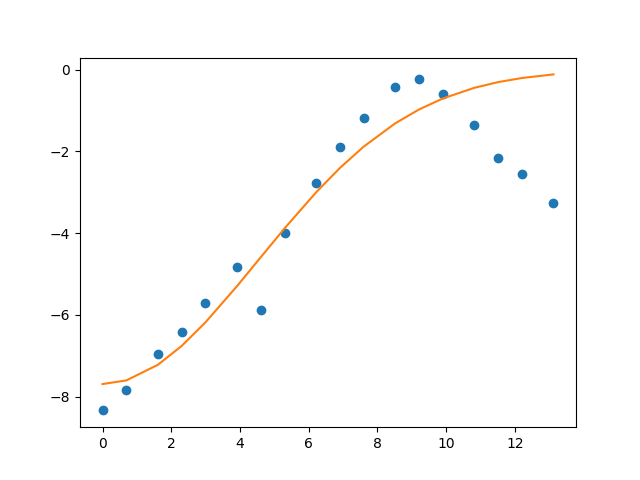
\includegraphics[scale=0.75]{Gaussian fit.png}
\end{center}
\end{latin}
فیت کردن  داده با تابع گاوسی ممکن نیست و خط رسم شده به داده‌ها فیت نشد. حال روش های دیگر را تست می‌کنیم. روش \lr{Cubic spline} در این روش بین هر دو نقطه یک خط با معادله‌ی مرتبه دوم فیت می‌کنیم:
\begin{latin}
\begin{Shaded}
\begin{Highlighting}[]
\ImportTok{import}\NormalTok{ matplotlib.pyplot }\ImportTok{as}\NormalTok{ plt}
\ImportTok{from}\NormalTok{ scipy.interpolate }\ImportTok{import}\NormalTok{ UnivariateSpline}
\ImportTok{import}\NormalTok{ numpy }\ImportTok{as}\NormalTok{ np}
\NormalTok{xdata }\OperatorTok{=}\NormalTok{ np.log(R)}
\NormalTok{ydata }\OperatorTok{=}\NormalTok{ np.log(I}\OperatorTok{*}\NormalTok{V)}
\NormalTok{s }\OperatorTok{=}\NormalTok{ UnivariateSpline(xdata, ydata, s}\OperatorTok{=}\DecValTok{5}\NormalTok{)}
\NormalTok{xs }\OperatorTok{=}\NormalTok{ np.linspace(}\DecValTok{0}\NormalTok{, }\DecValTok{15}\NormalTok{, }\DecValTok{100}\NormalTok{)}
\NormalTok{ys }\OperatorTok{=}\NormalTok{ s(xs)}
\NormalTok{plt.plot(xdata, ydata, }\StringTok{\textquotesingle{}o\textquotesingle{}}\NormalTok{)}
\NormalTok{plt.plot(xs, ys)}
\NormalTok{plt.show()}
\end{Highlighting}
\end{Shaded}
\begin{center}
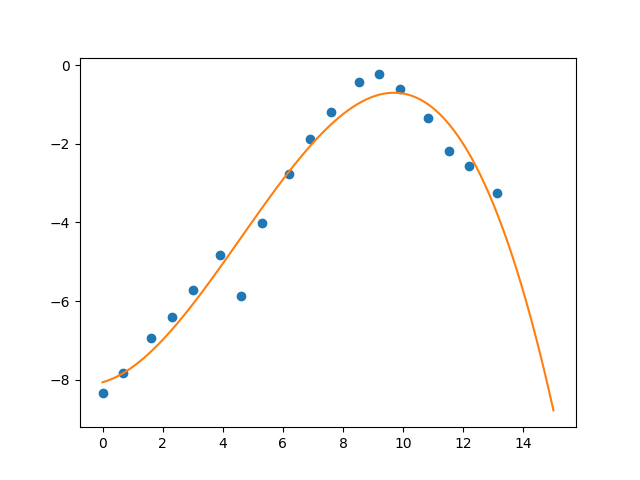
\includegraphics[scale=0.75]{Spline fit.png}
\end{center}
\end{latin}
خط رسم شده به نمودار فیت شد. \\
برای آنکه اطمینان بیشتری حاصل شود، توابع چند جمله‌ای از مراتب دو تا هفت را در دو پلات جداگانه به داده‌ها فیت می‌کنیم:
\begin{latin}
\begin{Shaded}
\begin{Highlighting}[]
\ImportTok{import}\NormalTok{ numpy }\ImportTok{as}\NormalTok{ np}
\ImportTok{import}\NormalTok{ matplotlib.pyplot }\ImportTok{as}\NormalTok{ plt}
\ImportTok{from}\NormalTok{ scipy.optimize }\ImportTok{import}\NormalTok{ curve\_fit}
\CommentTok{\#\# x{-}axis for the plot}
\NormalTok{xdata }\OperatorTok{=}\NormalTok{ np.log(R)}
\NormalTok{ydata }\OperatorTok{=}\NormalTok{ np.log(I}\OperatorTok{*}\NormalTok{V)}
\NormalTok{plt.scatter(xdata, ydata)}
\NormalTok{model2 }\OperatorTok{=}\NormalTok{ np.poly1d(np.polyfit(xdata, ydata, }\DecValTok{2}\NormalTok{))}
\NormalTok{polyline }\OperatorTok{=}\NormalTok{ np.linspace(}\DecValTok{1}\NormalTok{, }\DecValTok{15}\NormalTok{, }\DecValTok{50}\NormalTok{)}
\NormalTok{plt.scatter(xdata, ydata)}
\NormalTok{plt.plot(polyline, model2(polyline),  }\StringTok{\textquotesingle{}{-}\textquotesingle{}}\NormalTok{, label}\OperatorTok{=}\StringTok{\textquotesingle{}quadratic\textquotesingle{}}\NormalTok{)}
\NormalTok{model3 }\OperatorTok{=}\NormalTok{ np.poly1d(np.polyfit(xdata, ydata, }\DecValTok{3}\NormalTok{))}
\NormalTok{polyline }\OperatorTok{=}\NormalTok{ np.linspace(}\DecValTok{1}\NormalTok{, }\DecValTok{15}\NormalTok{, }\DecValTok{50}\NormalTok{)}
\NormalTok{plt.scatter(xdata, ydata)}
\NormalTok{plt.plot(polyline, model3(polyline),  }\StringTok{\textquotesingle{}{-}\textquotesingle{}}\NormalTok{, label}\OperatorTok{=}\StringTok{\textquotesingle{}cubic\textquotesingle{}}\NormalTok{)}
\NormalTok{model4 }\OperatorTok{=}\NormalTok{ np.poly1d(np.polyfit(xdata, ydata, }\DecValTok{4}\NormalTok{))}
\NormalTok{polyline }\OperatorTok{=}\NormalTok{ np.linspace(}\DecValTok{1}\NormalTok{, }\DecValTok{15}\NormalTok{, }\DecValTok{50}\NormalTok{)}
\NormalTok{plt.scatter(xdata, ydata)}
\NormalTok{plt.plot(polyline, model4(polyline),  }\StringTok{\textquotesingle{}{-}\textquotesingle{}}\NormalTok{, label}\OperatorTok{=}\StringTok{\textquotesingle{}Fourth degree\textquotesingle{}}\NormalTok{)}
\NormalTok{plt.legend()}
\NormalTok{plt.show()}
\end{Highlighting}
\end{Shaded}
\begin{center}
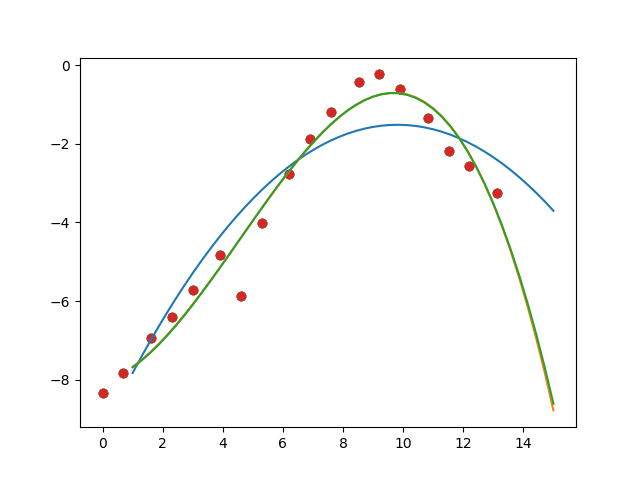
\includegraphics[scale=0.75]{quadratic, cubic, Fourth degree, curve fit.png}	
%\caption{توابع چند جمله‌ای مرتبه دوم سوم و چهارم به داده‌ها فیت شده‌‌اند.}
\end{center}
\end{latin}
همانطور که در شکل بالا دیده می‌شود، هیچ یک از توابع مرتبه دوم و سوم و چهارم یک خط فیت شده به صورت رضایت بخش به ما ارائه نداده است.(خطوط مرتبه سوم و چهارم منطبق به یکدیگر است.)
\begin{latin}
\begin{Shaded}
\begin{Highlighting}[]
\ImportTok{import}\NormalTok{ numpy }\ImportTok{as}\NormalTok{ np}
\ImportTok{import}\NormalTok{ matplotlib.pyplot }\ImportTok{as}\NormalTok{ plt}
\ImportTok{from}\NormalTok{ scipy.optimize }\ImportTok{import}\NormalTok{ curve\_fit}
\CommentTok{\#\# x{-}axis for the plot}
\NormalTok{xdata }\OperatorTok{=}\NormalTok{ np.log(R)}
\NormalTok{ydata }\OperatorTok{=}\NormalTok{ np.log(I}\OperatorTok{*}\NormalTok{V)}
\NormalTok{model5 }\OperatorTok{=}\NormalTok{ np.poly1d(np.polyfit(xdata, ydata, }\DecValTok{5}\NormalTok{))}
\NormalTok{polyline }\OperatorTok{=}\NormalTok{ np.linspace(}\DecValTok{1}\NormalTok{, }\DecValTok{15}\NormalTok{, }\DecValTok{50}\NormalTok{)}
\NormalTok{plt.scatter(xdata, ydata)}
\NormalTok{plt.plot(polyline, model5(polyline),  }\StringTok{\textquotesingle{}{-}\textquotesingle{}}\NormalTok{, label}\OperatorTok{=}\StringTok{\textquotesingle{}Fifth degree\textquotesingle{}}\NormalTok{)}
\NormalTok{model6 }\OperatorTok{=}\NormalTok{ np.poly1d(np.polyfit(xdata, ydata, }\DecValTok{6}\NormalTok{))}
\NormalTok{polyline }\OperatorTok{=}\NormalTok{ np.linspace(}\DecValTok{1}\NormalTok{, }\DecValTok{15}\NormalTok{, }\DecValTok{50}\NormalTok{)}
\NormalTok{plt.scatter(xdata, ydata)}
\NormalTok{plt.plot(polyline, model6(polyline),  }\StringTok{\textquotesingle{}{-}\textquotesingle{}}\NormalTok{, label}\OperatorTok{=}\StringTok{\textquotesingle{}sixth degree\textquotesingle{}}\NormalTok{)}
\NormalTok{model7 }\OperatorTok{=}\NormalTok{ np.poly1d(np.polyfit(xdata, ydata, }\DecValTok{7}\NormalTok{))}
\NormalTok{polyline }\OperatorTok{=}\NormalTok{ np.linspace(}\DecValTok{1}\NormalTok{, }\DecValTok{15}\NormalTok{, }\DecValTok{50}\NormalTok{)}
\NormalTok{plt.scatter(xdata, ydata)}
\NormalTok{plt.plot(polyline, model7(polyline),  }\StringTok{\textquotesingle{}{-}\textquotesingle{}}\NormalTok{, label}\OperatorTok{=}\StringTok{\textquotesingle{}seventh degree\textquotesingle{}}\NormalTok{)}
\NormalTok{plt.legend()}
\NormalTok{plt.show()}
\end{Highlighting}
\end{Shaded}
\begin{center}
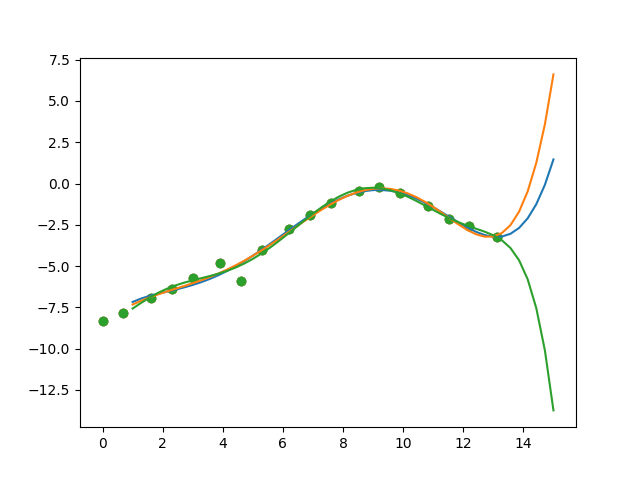
\includegraphics[scale=0.75]{fifth degree, sixth degree, seventh degree, curve fit.png}
\end{center}
\end{latin}

خطوط رسم شده توسط هر‌سه معادله‌ی مرتبه‌ پنجم و ششم و هفتم به بهترین شکل ممکن به داده‌ها فیت شد. فرمول هریک از خطوط زیر به شکل زیر است:

\begin{latin}

quadratic Ep:\\      
$-0.08125 x^2 + 1.595 x - 9.341$\\
cubic Eq:\\   
$-0.0139 x^3 + 0.1913 x^2 + 0.2119 x - 8.063$\\
Fourth degree Eq:\\
$7.066e-05 x^4 - 0.01576 x^3 + 0.2066 x^2 + 0.1702 x - 8.043$\\
Fifth degree Eq:\\
$0.0006476 x^5 - 0.02122 x^4 + 0.2301 x^3 - 0.9615 x^2 + 2.139 x - 8.558$\\
sixth degree Eq:\\
$4.977e-05 x^6 - 0.001319 x^5 + 0.007978 x^4 + 0.02954 x^3 - 0.335 x^2 + 1.424 x - 8.452$\\
seventh degree Eq:\\
$-2.781e-05 x^7 + 0.001326 x^6 - 0.02434 x^5 + 0.2144 x^4 - 0.9245 x^3 + 1.773 x^2 - 0.3043 x - 8.306$\\
\end{latin}



	
3.با توجه به اندازه‌گیری‌های بخش‌های پیشین برای $I_{sc}$ و $V_{oc}$ و $I_{mpp}$ و $V_{mpp}$ سازه‌ی پرشدگی و خطای آن را محاسبه کنید. \\
\textbf{خطاگیری در پیوست به صورت دست نویس قرار گرفته است.}
	
	4.با کمک یک میزچه‌ی مدرج تغییرات $I$ را به صورت تابعی از زاویه‌ی فرود در فاصله‌ی ثابتی از لامپ اندازه‌گیری کنید. ونمودار تغییرات $I$ بر حسب $\cos^2 {\theta}$ را رسم کنید. آیا رابطه خطی است؟ علت آن را بنویسید.
	
\begin{latin}
\vspace{3cm}
\begin{center}
\begin{table}[h!]
\centering
\setlength{\tabcolsep}{8pt}
\renewcommand{\arraystretch}{2}
\begin{tabular}{|c|c|c|c|c|c|c|c|c|c|c|}
\hline
\multicolumn{11}{|c|}{Changes in current according to the change of landing angle} \\
\hline
$\theta$&0&10&20&30&40&50&60&70&80&90\\
\hline
$I\pm0.001mA$&0.086&0.083&0.079&0.077&0.068&0.059&0.050&0.038&0.021$\pm$0.003mA&0.013$\pm$0.003mA\\
\hline
\end{tabular}
\caption{}
\end{table}
\end{center}
\end{latin}


\begin{latin}
\hypertarget{i-cos2theta}{%
\section{I-cos\^{}2(theta)}\label{i-cos2theta}}
\begin{Shaded}
\begin{Highlighting}[]
\ImportTok{import}\NormalTok{ matplotlib.pyplot }\ImportTok{as}\NormalTok{ plt}
\ImportTok{import}\NormalTok{ seaborn }\ImportTok{as}\NormalTok{ sns}
\ImportTok{import}\NormalTok{ numpy }\ImportTok{as}\NormalTok{ np}
\ImportTok{from}\NormalTok{ math }\ImportTok{import}\NormalTok{ pi}
\ImportTok{import}\NormalTok{ pandas }\ImportTok{as}\NormalTok{ pd}
\ImportTok{import}\NormalTok{ scipy}
\NormalTok{I\_o }\OperatorTok{=}\NormalTok{ np.array([}\FloatTok{0.086}\NormalTok{, }\FloatTok{0.083}\NormalTok{, }\FloatTok{0.079}\NormalTok{, }\FloatTok{0.077}\NormalTok{, }\FloatTok{0.068}\NormalTok{, }\FloatTok{0.059}\NormalTok{, }\FloatTok{0.050}\NormalTok{, }\FloatTok{0.038}\NormalTok{, }\FloatTok{0.021}\NormalTok{, }\FloatTok{0.013}\NormalTok{])}
\NormalTok{theta }\OperatorTok{=}\NormalTok{ np.array([}\DecValTok{0}\NormalTok{, pi}\OperatorTok{/}\DecValTok{18}\NormalTok{, pi}\OperatorTok{/}\DecValTok{9}\NormalTok{, pi}\OperatorTok{/}\DecValTok{6}\NormalTok{, }\DecValTok{40}\OperatorTok{*}\NormalTok{pi}\OperatorTok{/}\DecValTok{180}\NormalTok{, }\DecValTok{50}\OperatorTok{*}\NormalTok{pi}\OperatorTok{/}\DecValTok{180}\NormalTok{, pi}\OperatorTok{/}\DecValTok{3}\NormalTok{, }\DecValTok{70}\OperatorTok{*}\NormalTok{pi}\OperatorTok{/}\DecValTok{180}\NormalTok{, }\DecValTok{80}\OperatorTok{*}\NormalTok{pi}\OperatorTok{/}\DecValTok{180}\NormalTok{, pi}\OperatorTok{/}\DecValTok{2}\NormalTok{])}
\NormalTok{cos2 }\OperatorTok{=}\NormalTok{ np.cos(theta)}\OperatorTok{**}\DecValTok{2}
\NormalTok{df }\OperatorTok{=}\NormalTok{ pd.DataFrame(\{}\StringTok{\textquotesingle{}cosine\_by\_power\_of\_two\textquotesingle{}}\NormalTok{:cos2, }\StringTok{\textquotesingle{}I\textquotesingle{}}\NormalTok{:I\_o\})}
\CommentTok{\#create regplot}
\NormalTok{p }\OperatorTok{=}\NormalTok{ sns.regplot(data}\OperatorTok{=}\NormalTok{df, x}\OperatorTok{=}\NormalTok{df.cosine\_by\_power\_of\_two, y}\OperatorTok{=}\NormalTok{df.I)}
\CommentTok{\#calculate slope and intercept of regression equation we use slop and intercept in equation}
\NormalTok{slope, intercept, r, p, sterr }\OperatorTok{=}\NormalTok{ scipy.stats.linregress(x}\OperatorTok{=}\NormalTok{p.get\_lines()[}\DecValTok{0}\NormalTok{].get\_xdata(),}
\NormalTok{                                                       y}\OperatorTok{=}\NormalTok{p.get\_lines()[}\DecValTok{0}\NormalTok{].get\_ydata())}
\CommentTok{\#add regression equation to plot}
\NormalTok{equation2 }\OperatorTok{=} \StringTok{\textquotesingle{}y = \textquotesingle{}} \OperatorTok{+} \BuiltInTok{str}\NormalTok{(}\BuiltInTok{round}\NormalTok{(intercept,}\DecValTok{3}\NormalTok{)) }\OperatorTok{+} \StringTok{\textquotesingle{} + \textquotesingle{}} \OperatorTok{+} \BuiltInTok{str}\NormalTok{(}\BuiltInTok{round}\NormalTok{(slope,}\DecValTok{3}\NormalTok{)) }\OperatorTok{+} \StringTok{\textquotesingle{}x\textquotesingle{}}
\CommentTok{\# plt.plot(cos2, I\_o)}
\NormalTok{plt.legend()}
\NormalTok{plt.show()}
\end{Highlighting}
\end{Shaded}
\begin{center}
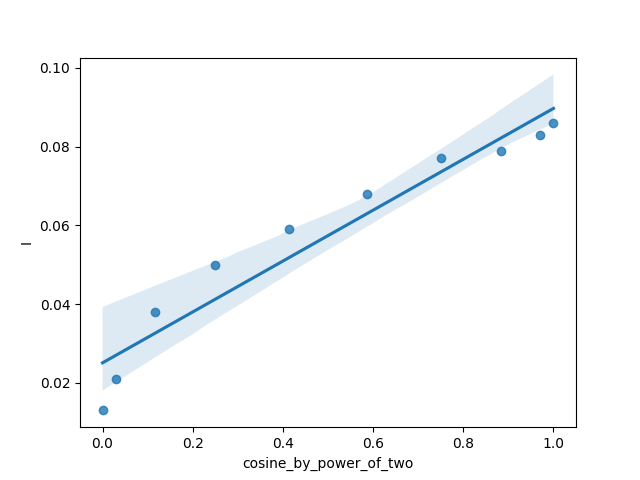
\includegraphics[scale=0.80]{I-cos^2(theta) fig.png}
\end{center}
\end{latin}
معادله‌ی خط فیت شده به صورت زیر است:
\begin{latin}
\begin{Highlighting}
\BuiltInTok{print}\NormalTok{(}\SpecialStringTok{F"Eq2: }\SpecialCharTok{\{}\NormalTok{equation2}\SpecialCharTok{\}}\SpecialStringTok{"}\NormalTok{)}
\end{Highlighting}
\begin{verbatim}
Eq2: y = 0.025 + 0.065x
\end{verbatim}	
\end{latin}

\section{پرسش‌ها}
1. چگونگی ساخت نیم‌رسانا‌های گونه‌ی n و گونه‌ی p را شرح دهید.\\
\paragraph{پاسخ} برای تشکیل نیم‌رسانا نیاز به حداقل دو‌‌گونه اتم داریم.
یک گونه از این اتم‌ها باید دارای $t$ الکترون ظرفیت(اتم A) و دیگری باید شامل $t+1 $الکترون ظرفیت (اتم B) باشد. در این صورت، اگر در یک شبکه از اتم‌های A و B، به طور تکراری، یک اتم B با $t$ اتم A پیوند برقرار ‌کند؛اتمB دارای یک الکترون ظرفیت آزاد می‌ماند. این  شبکه‌ی تشکیل شده یک نیم‌رسانای نوع n است.\\
به طور مشابه می‌توان، یک گونه از این اتم‌ها باید دارای $t$ الکترون ظرفیت(اتم A) و دیگری باید شامل $t-1 $الکترون ظرفیت (اتم C) باشد. در این صورت، اگر در یک شبکه از اتم‌های C و A، به طور تکراری، یک اتم C با $t-1$ اتم A پیوند برقرار ‌کند؛اتم C در شبکه، یک حفره تشکیل می‌دهد‌. شبکه‌ی تشکیل شده یک نیم‌رسانای نوع p است.\\

با ترکیب این سه مدل اتم با یکدیگر، این حفره‌ها و الکترون‌ها تشکیل یک نیم رسانا می‌دهند. \\
2. مراحل تبدیل انرژی نورانی به انرژی الکتریکی را در یک باتری خورشیدی توضیح دهید.\\
3. خطاهای موجود در آژمایش را بیان کنید و در صورت امکان راه حلی برای کاهش آن‌ها بیابید.\\
4. هم‌ارزی دو تعریف داده شده بریا جریان اتصال کوتاه را نشان دهید.\\
5. آیا اندازه‌گیری جریان اتصال کوتاه در بخش اول آزمایش این جریان را به درستی نشان می‌دهد؟ دلیل آن را بیان کنید.\\
6. آیا ولتاژ مدار بازی که به دست می‌آورید با تعریف نظری آن هم خوانی دارد؟ چرا؟\\

ت یافتن نقطه ماکزیمم ای و وی
	
	
	
	
	
	
	
	
	
\end{document}